\documentclass{article}
\usepackage[utf8]{inputenc}
\usepackage{tabu}
\usepackage{graphicx}

\title{Elaboration I & II}
\author{Sophie Avard }
\date{August/September 2019}

\begin{document}

\maketitle

\tableofcontents
\pagebreak

\section{Introduction}
\begin{center}
\textit{Elaboration addresses major risks, builds on an early skeleton architecture of the system, and redefines and evilest the project plans (Kroll and Kruchten, 2003)}.
\end{center}

Using Kroll and Kruchten’s (2003) Elaboration Phase as a framework, I will identify technologies and other components of modern data collection that could accomplish each step of my POC. In addition, I will also address problems that may arise and will provide alternative solutions. The Elaboration Plan will divided into three stages:
\begin{enumerate}
    \item A detailed understanding of the requirements
    \item Architecture design 
    \item Risks and solutions
\end{enumerate}

\section{Requirements}
During the Scoping exercise, I focused on developing a tool to manage multiple sources of data collected during field work. That is, the tool would identify particular themes and reoccurring patterns within data that has been rendered in one format. For instance, Anthropologists use a variety of methodologies to collect data - such as online sources, audio recordings, interviews, questionnaires, focus groups and participant observation. Following data collection, key words and meaningful chunks of information are extracted from the data - this is called coding. Codes provide both inspiration and verification as they discover significant categories and relationships within dense and saturated data. 

\subsection{Open Coding}
Open coding is the initial analysis phase. It involves identifying codes without any restrictions or purpose other than to discover chunks of meaning. Open coding requires researcher's to be open in order to make unexpected discoveries and to refrain from closure even after codes have been identified. As open coding is concerned with labelling and categorising phenomena, the constant comparative method may be used to continuously compare each piece of data with codes already identified. This helps identity distinct characteristics and ordinal positions of relevant scales. When theoretical saturation is achieved - When no further codes or categories can be identified - a process called sorting or ordering data taking place. This involves identifying contrasts and relationships between codes, such as indicating particular outliers and the frequency of codes. 

\subsection{Axial Coding}
Axial coding refers to discovering codes around a single category in order to discover links and relationships. For example, in a category of 'greeting' there may be a search for encounters with other people, talk about previous encounters and emotional impacts from meeting others. Axial coding looks for:
\begin{itemize}
    \item Causal conditions
    \item Contextual factors
    \item Actions and interactions taken in response to the phenomena
    \item Intervening conditions that assist or hinder actions and interactions
    \item Consequences of actions and interactions
\end{itemize}
Axial coding may be done at any time, even prior to identifying firm categories. For example, when a code of 'rain' is first encountered, then an exploration of the impacts and importance of rain may ensue. Axial coding also helps identify relationships and the links that create a web of meaning for the people under study.

\subsection{Selective Coding}
Selective coding focuses on core categories in order to identify specific links and how these links may or may not lie at the heart of the matter. This helps with organising and integrating categories. 

\section{Architecture}
Identifying codes and categories is a long and exhaustive process of repeated word-by-word analysis. The problem here is that more data leads to better categories, theories and conclusions, however more data also requires more effort and time. Therefore, this technology deployment will involve using R to perform analyses like free-list and pile sort. As such, the architecture design can be broken into two main components:
\begin{enumerate}
\item CAQDAS: ATLAS.ti, NVivo and RQDA -  this will identify types and levels of meaningful phenomena.
\item Cultural Domain Analysis: ANTHROPAC and AnthroTools -  this will be used to gain insight into the importance and association between codes and categories.
\end{enumerate}
In order to implement this script in R, an architecture must first be designed, validated and tested. Architecture refers to the building blocks and skeleton of the structure of the software design. This does not involve complete functionality, but rather it will:
\begin{enumerate}
    \item Select the technologies, main components and their interfaces
    \item Plan the execution for each step
    \item Implement architectural mechanisms through identifying possible alternate routes.
\end{enumerate}
While this phase has three components that need to be addressed, only one will be discussed in Elaboration I. Firstly, the most important building blocks of the system, and their interfaces, as well as the decision to build or reuse some of these building blocks will be identified. Secondly, how these building blocks will interact at run-time to implement the most important components will be described. The last component involves a prototype of this architecture to validate that it does work, that the major technical risks are resolved, and that it has the proper quality attributes: performance, scalability, and cost. The last two components: Interaction and Implementation will be tested in during Elaboration II.

\subsection{Building Blocks}
This processes will identify technologies (programming languages, software libraries, APIs) and other components of a modern data collection or processing workflow that could accomplish each step.

\setlength{\parindent}{0em}
\setlength{\parskip}{1em}
\begin{center}
\textbf{Computer-assisted qualitative data analysis software (CAQDAS)}
\end{center}

\subsubsection{ATLAS.ti}
ATLAS.ti could offer a variety of tools for accomplishing the tasks associated with data that cannot be meaningfully analysed by formal, statistical approaches. ATLAS.ti could also help with managing, extracting and exploring the data as it keeps all the data, codes, memos, and findings in a single environment. Moreover, the software can help with creating a graphical view of the data and relevant concepts. However, the software only helps organises data, it does not analyse the data. 

\subsubsection{NVivo}
NVivo is proprietary software that provides users with one-click access to word frequencies and key words in context, allowing the identification of patterns across various data sources. NVivo can help discover connections and deeper insights. NVivo claims it can conduct text searches, word frequency queries and help with thematic analyses. NVivo would be useful if it does what it claims to do:
\begin{itemize}
    \item Work with a variety of text and data sources (interview transcripts, journal articles, images, web content and videos.
    \item Organise, store and retrieve data.
    \item Conduct text searches and word counts through word frequency queries. 
    \item Group words according to synonyms and other lexical associations.
    \item Examine themes and structure data.
    \item Visualise the findings.
\end{itemize}

\subsubsection{RQDA}
RQDA is open-source software (OSS). Unlike ATLAS.ti and NVivo, RQDA users have open access to the source code and are able to use it in any way they see fit. However, RQDA does not provide technical support from its developer, it only supports text (.txt) and it does not support multimedia files. While RQDA only offers a two-level code aggregation to support research, the simple yet efficient data aggregation function enables research to be the main driver of the theory-building process.

\begin{tabu} to 1.0\textwidth { | X[l] | X[l] | X[l]| X[l]|}
 \hline
 \textbf{Aspect of comparison} & \textbf{RQDA} & \textbf{ATLAS.ti} & \textbf{NVivo} \\
 \hline
 License  & Open source  & proprietary & proprietary  \\
\hline
File compatibility & .txt only & audio, graphic, text, video & audio, graphic, text, video \\
\hline
Language & allow import data in Indonesia & doesnt allow Indonesian & doesnt allow Indonesian\\
\hline 
Statistical functions & enables users to write R commands for statistical analysis and apply various R packages for statistical analysis under a single platform & enable data to be transformed into tabulations & enable data to be transformed into tabulations\\
\hline
Code aggregation & up to two levels of hierarchical structure of coding & limited to no function for hierarchical structure of coding & good function for hierarchical structure of coding\\
\hline Output sharing & HTML file & SPSS and XML & RTF, Excel and HTML table \\
\hline 
Methodological material & .txt files & all file types & all file types\\
\hline
\end{tabu}

\setlength{\parindent}{0em}
\setlength{\parskip}{1em}

While ATLAS.ti and NVivo enable data attributes to be transformed into tabulations for further statistical analysis, I have chosen to use RQDA for the following reasons:
\begin{itemize}
    \item It is open source software
    \item It allows users to write R syntax to conduct statistical analysis of numerous textual files. 
    \item It allows data to be imported in Indonesian 
\end{itemize}

If RQDA fails to do what my analysis requires, I will use NVivo. This is purely because ATLAS.ti only exports data in SPSS and XML format.

\begin{center}
\textbf{Cultural Domain Analysis}
\end{center}
If RQDA and NVivo cannot provide appropriate anthropological analyses such as open coding and axial coding, then techniques for cultural domain analysis may be used. Cultural domain analysis describes contents, structure, and distribution of knowledge in organised spheres of experience.

\subsubsection{ANTHROPAC} 
ANTHROPAC is a software program from analysing data on cultural domains. It helps collect and analyse structured qualitative data including free-lists, pile-sorts, triads, paired comparisons, and ratings. Furthermore, ANTHROPAC provides a variety of data manipulation tools, has a User's guide, and methods guide. However, ANTHROPAC requires data to be organised in a particular .txt file format. This method may become laborious if working with large amounts of data. 

\subsubsection{AnthroTools}
AnthroTools allows researchers to quickly analyse free-list data and convert it into various datasets that are more immediately useable. Moreover, AnthroTools uses the open-source program R that will be used for CAQDAS. The free-list analysis tool will allow me to calculate the salience of specific concepts that arise during interviews. If successful, this tool would allow me to assess the structure of the participants thoughts and the way they conceptualise particular concepts. However, this tool requires participants to list objects in a given domain. As interviews are semi-structured, this process may be hard.

\section{Risks and Solutions}
The risks and appropriate solutions are as follows:

\subsection{Legal and financial issues}
This issues related to the usage of open source or commercial components. In order to mitigate financial strain only open source software will be used (Eg. RQDA).

\subsection{Solving the easy stuff first}
In order to avoid hasty solutions and decision making, I will tackle the hard issues first. This will be done through continuously updating my risk list in order to guide my focus towards the biggest risks. first. 

\subsection{Falling behind schedule}
In order to prevent the project from falling behind schedule it is important to have each phase uploaded to CloudStor on time.

\subsection{Ending elaboration before the architecture is stable}
This will cause excessive re-work and lower quality of work. Make sure that each component is tested and produces the desired results.

\section{Revision of POC}
After doing further research into the tools available, the processes involved, and the considering the time limits I have decided to focus on using R to develop a script for analysing and coding qualitative data - using methods such as free-list analysis and pile sorting. This will involve the following steps:
\begin{enumerate}
    \item Convert necessary data into .txt format
    \item Import the files on R 
    \item Run the RQDA package on R 
    \item Run a word frequency analysis
    \item Use the frequency output to conduct open coding
    \item Use pile sort method to examine interactions and relationships between codes and categories (axial coding)
    \item Produce a coding table to get a descriptive look at the data.
    \item Export as HTML
\end{enumerate}
If RQDA doesn't produce appropriate coding analysis:
\begin{enumerate}
    \item Add AnthroTools package to R \item Run a free-list analysis
    \item Run a salience calculation 
    \item Export in spreadsheet format
\end{enumerate}

\section{Elaboration Part II}
This phase involves implementing and evaluating the architecture previously listed. Firstly, I will test the tools to make sure they perform what is expected of them. If they do not do what I need them to do, I will try an alternative tool. This will continue until I find a tool that is able to perform the coding and analysis that is needed. After this, I will Revise my POC in light of the implementation results. 

\subsection{RQDA}
Steps completed:
\begin{enumerate}
    \item Covert transcript into .txt format by online text converter 
    % https://document.online-convert.com/convert-to-txt
    \item add the .txt file to my working directory
    \item Download R 
    \item Download R Studio - this makes it easier and more efficient 
    \item Follow to installation steps for RQDA (see learning journal)
\end{enumerate}

Unfortunately I could not run the analysis that I wanted to run as I kept getting and error message in R that would not allow me to use the RQDA package. For this reason I will seek an alternate tool, however, I may still use RQDA if I can fix the error. 

\subsection{AnthroTools}
AnthroTools package to R:\\
\verb|install.packages("devtools")|\\
\verb|library("devtools")|\\
\verb|install_github('alastair-JL/AnthroTools')|\\
\verb|library(AnthroTools)|\\

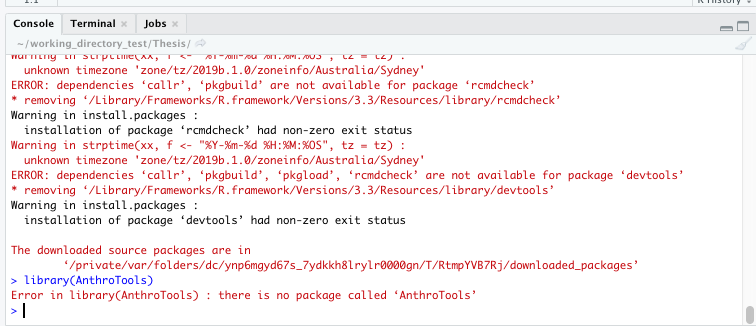
\includegraphics[width=\textwidth]{AnthroTools.png}

After installing to AnthroTools package I got another error message in R (see below image). It is clear that something is wrong on my end as I have been able to use AnthroTools previously. 

As such, I will test another alternative in case this cannot be fixed. 

\subsection{Voyant}
I implemented Voyant to see what type of textual analysis it would produce. I did this by uploading an essay that I have been working up for my thesis.

One of the requirements is a word frequency analysis. The results on Voyant successfully showed the frequency of terms used throughout the essay.

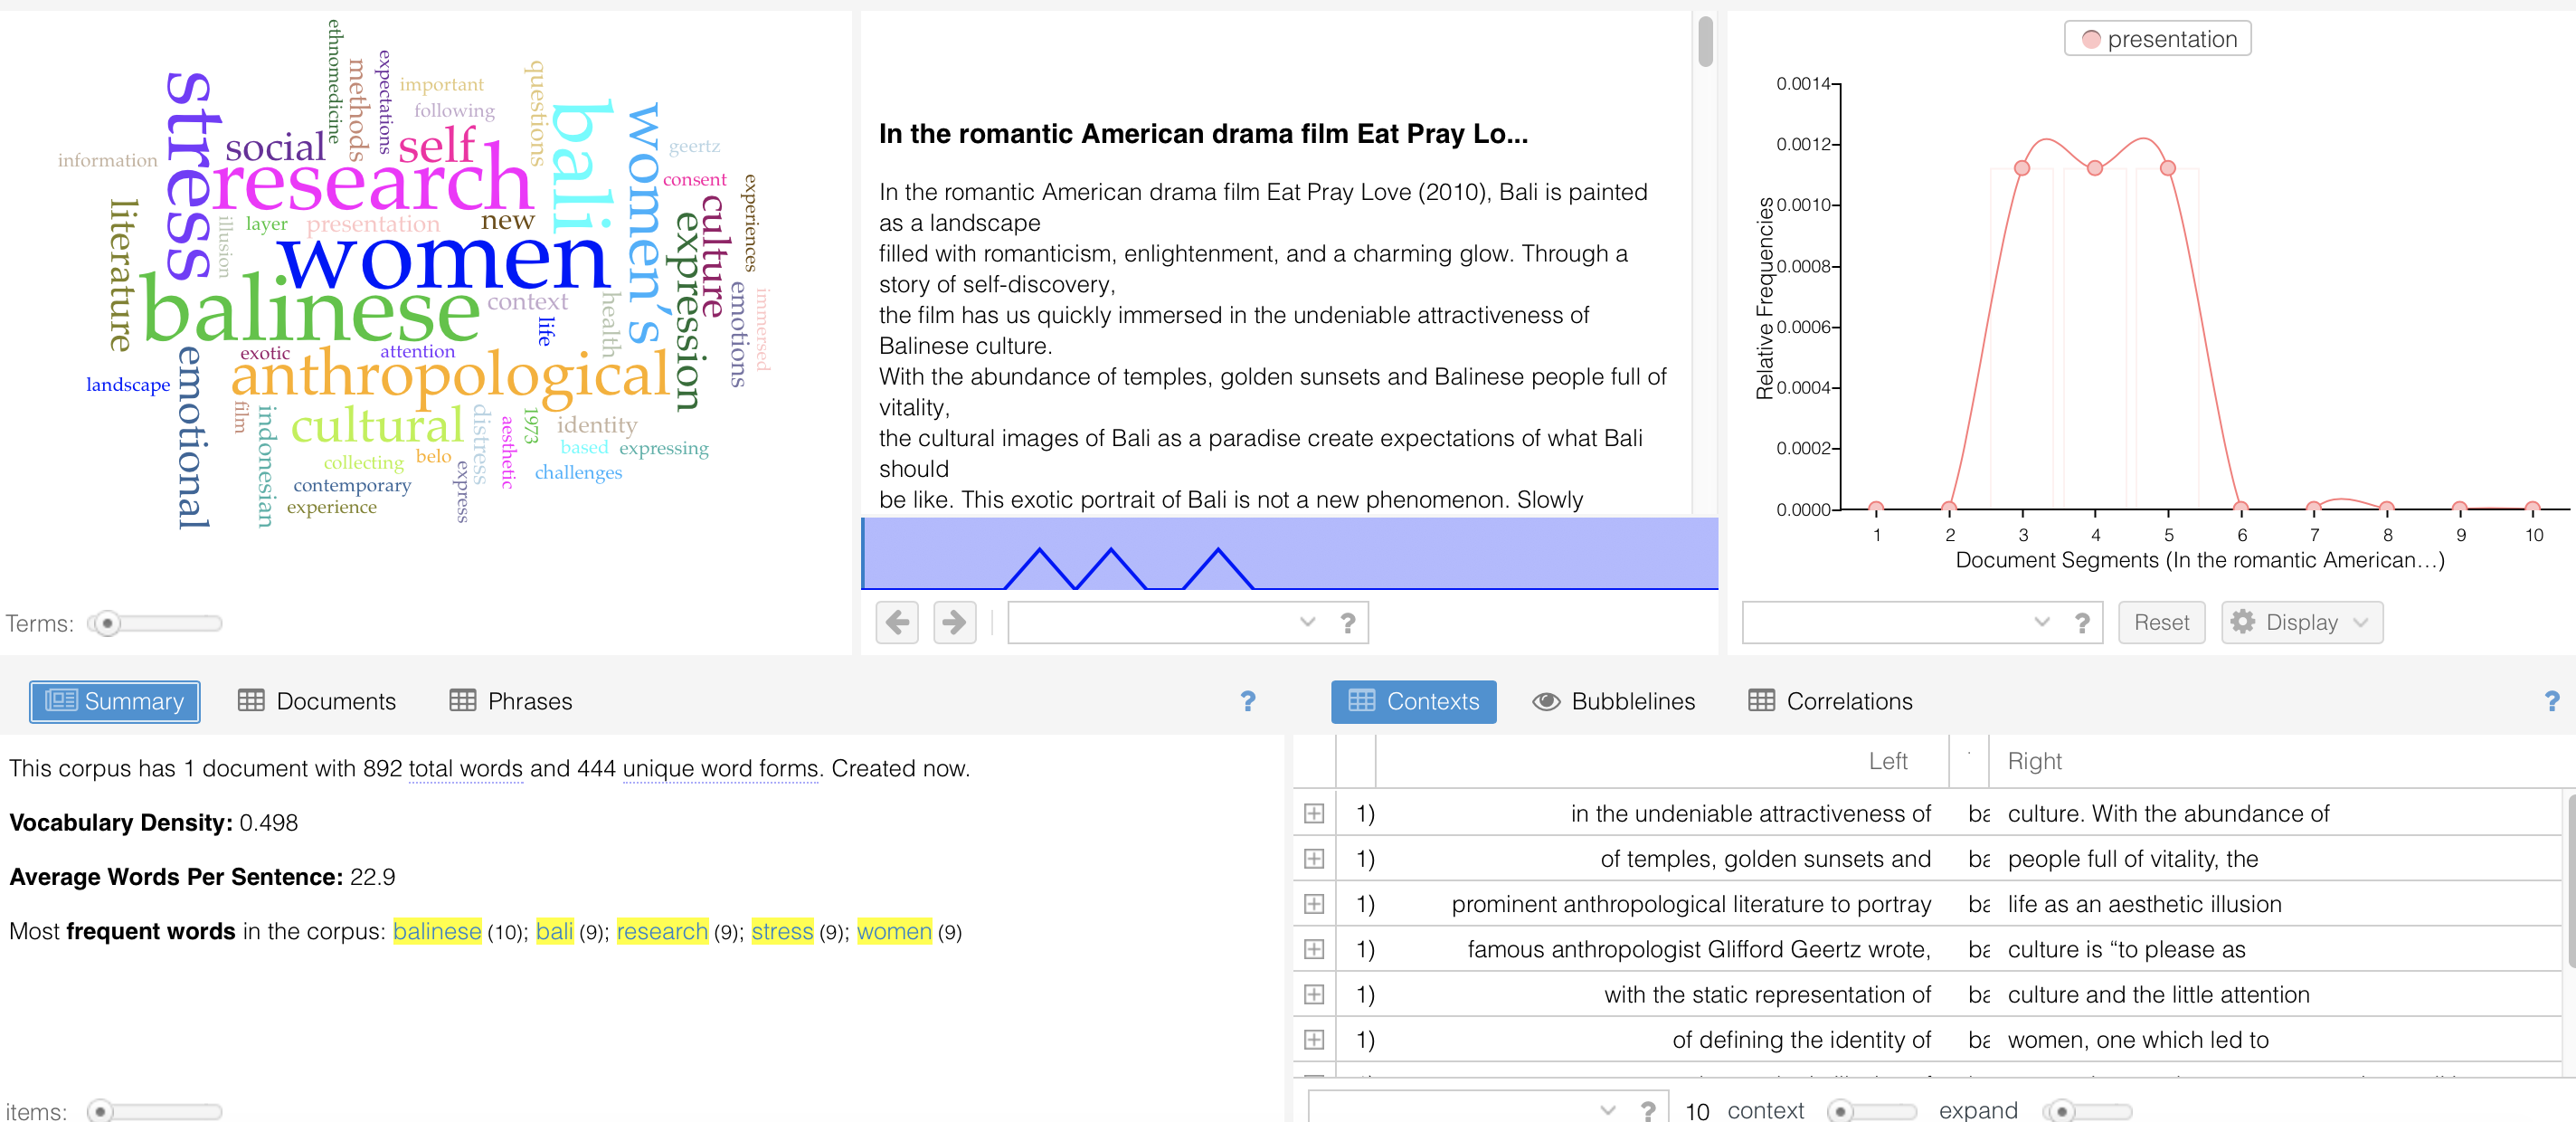
\includegraphics[width=\textwidth]{Voyant.png}

Another requirement of the analysis is discovering relationships between words/codes. Unfortunately Voyant did not provide this analysis.

While I think I will find a better tool, Voyant would still be useful for identifying the frequency of words within transcripts which then could be used for thematic coding. 

\subsection{ATLAS.ti}
After downloading ATLAS.ti, I uploaded two documents relevant to my thesis. A benefit of this tool is that you can upload most document types - eg. word, PDF, video, audio etc. I then added the following codes: 'stress', 'emotion', 'Bali', 'Balinese', Women' and conducted a word frequency analysis.  
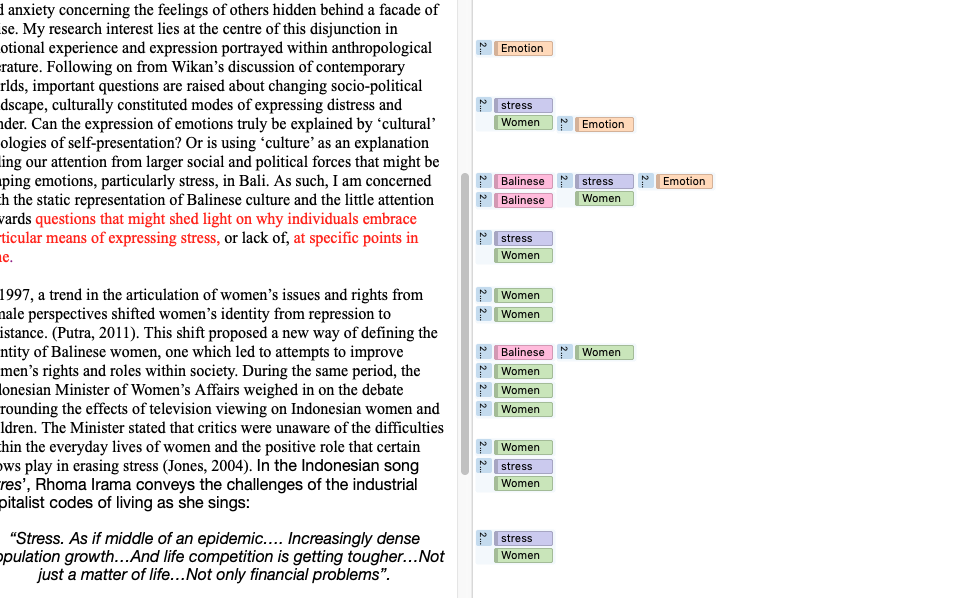
\includegraphics[width=\textwidth]{ATLAS.png}
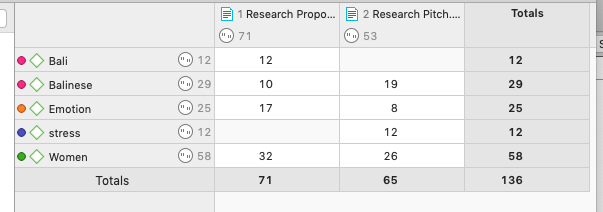
\includegraphics[width=\textwidth]{ATLAS2.png}

\subsection{NVivo}
NVivo is a well thought out tool. It has allows you to organise all your data within subfolders - eg. interviews, surveys, literature reviews - which can then be compared all in one place. It allowed me to upload a video from an interview I did a few years ago and I was also to attach the transcript to the video. 

In terms of analysis, it can do the following: word frequency, text search, code, and run comparison diagrams. The text search is useful because you can enter specific text and find matches that include stemmed words - such as "talk" and "talking". NVivo was also to create a relationship diagram with the codes related to particular sources - such as an interview. 

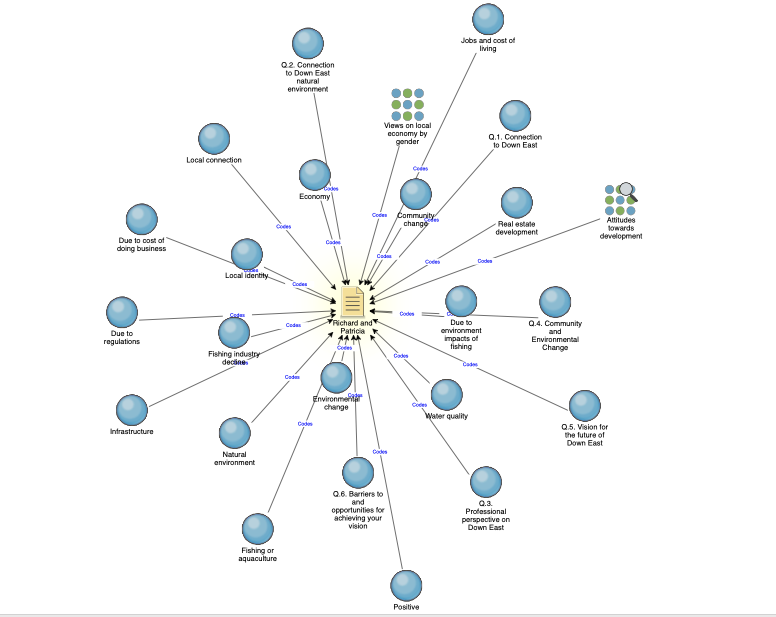
\includegraphics[width=\textwidth]{NVivo.png}

\section{Review of POC}
The tests that I implemented in elaboration II somewhat responded to the steps articulated in the first elaboration. The RQDA and AnthroTools tests were the only unsuccessful tools and this was due to an error on my end. This may be due to how I have downloaded R or how my computer is set up. Fortunately, Voyant, ATLAS.ti and NVivo were all successful at allowing my data to be coded and providing a word frequency analysis. While Nvivo was able to provide more insight in terms of thematic relationships and coding, I still believe that RQDA will provide a more useful analysis of my data

After doing tests on the tools available, the processes involved, and considering the time limits I have decided to focus on using RQDA in R to develop a script for analysing and coding qualitative data - using methods such as free-list analysis and pile sorting. This will involve the following steps:

that part of your testing is to get technical support with me before class, and based on that outcome, you'll adjust your plans

\begin{enumerate}
    \item Get technical support from Brian to fix error in R 
    \item Convert necessary data into .txt format
    \item Import the files on R 
    \item Run the RQDA package on R 
    \item Run a word frequency analysis
    \item Use the frequency output to conduct open coding
    \item Use pile sort method to examine interactions and relationships between codes and categories (axial coding)
    \item Produce a coding table to get a descriptive look at the data.
    \item Export as HTML
\end{enumerate}

\end{document}
